% Standalone annotated figure for R1.1 (particle-to-specimen size ratio)
%  (a) Full HCA specimen with wedge-marker location
%  (b) Detail of the marked wedge, with R-r dimension and d_max reference
% Blender geometry renders live in ../ .

\documentclass[border=5pt,tikz]{standalone}
\usepackage{tikz}
\usepackage{graphicx}
\usepackage{amsmath,amssymb}
\usetikzlibrary{positioning, calc, decorations.pathreplacing, arrows.meta}

\begin{document}

\begin{tikzpicture}[
    every node/.style={font=\small},
]

%% ── Image widths (cm) ──
\def\Wfull{6.0}
\def\Wdet{6.0}
\def\gap{0.5}

%% ── (a) Full HCA ──
\node[anchor=south west, inner sep=0] (full) at (0,0)
  {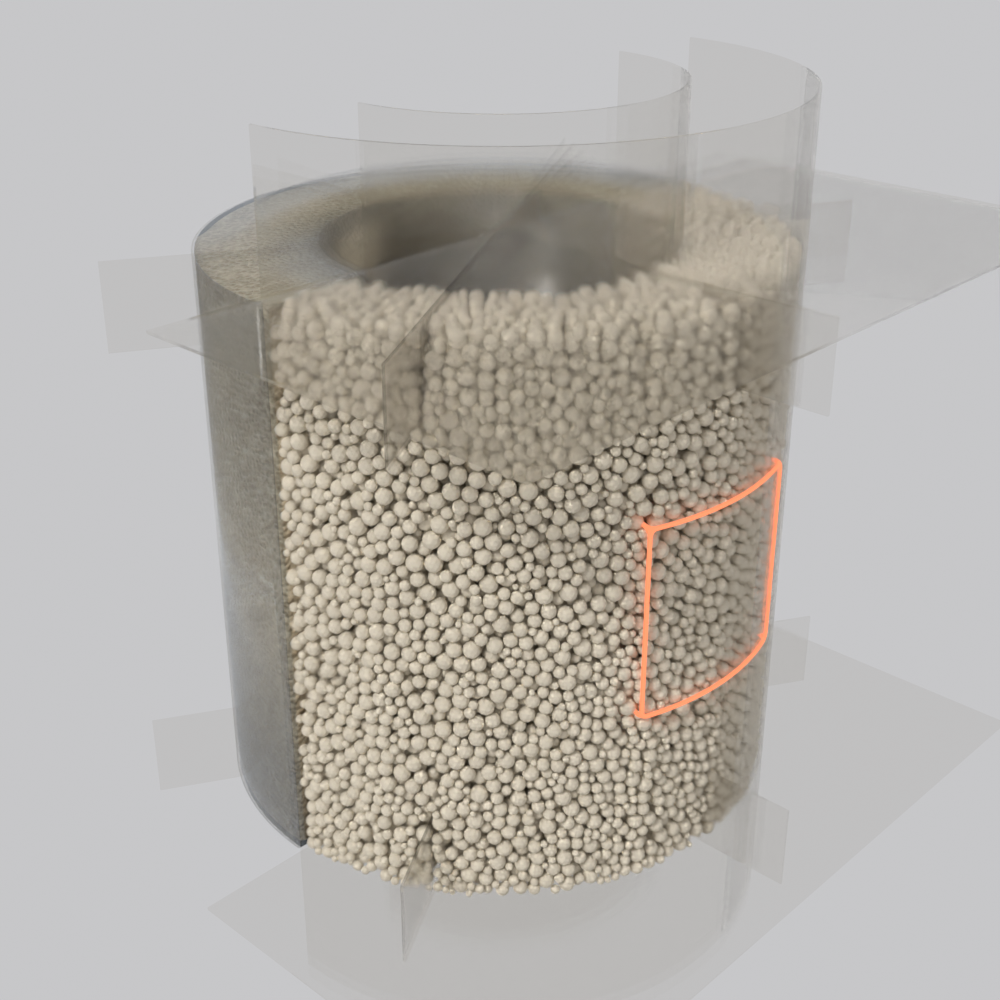
\includegraphics[width=\Wfull cm]{../rcell_full.png}};
\node[below=2pt of full.south] {\textbf{(a)} HCA specimen};

%% ── (b) Detail ──
\node[anchor=south west, inner sep=0] (det) at ({\Wfull + \gap},0)
  {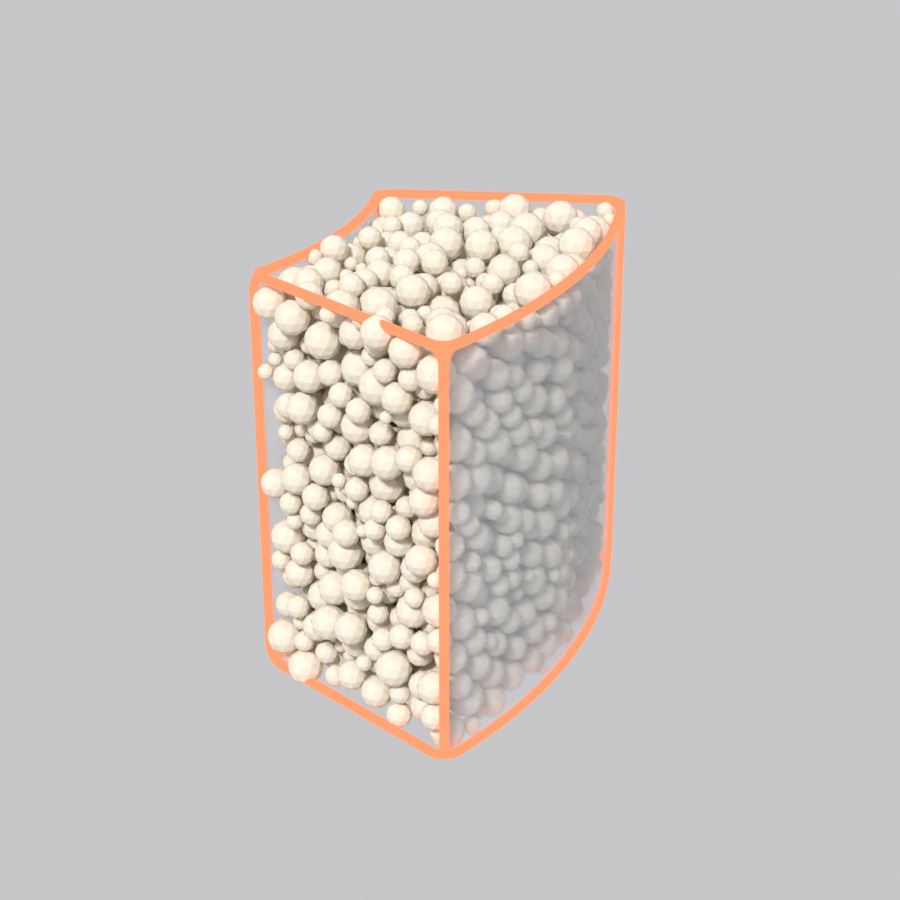
\includegraphics[width=\Wdet cm]{../rcell_detail.png}};
\node[below=2pt of det.south] {\textbf{(b)} Element detail};

%% ── Connector arrow from wedge-marker on (a) to (b) ──
% marker centre on (a): approx (0.72, 0.52) in normalized image coords
\coordinate (markA) at ($(full.south west) + (0.82*\Wfull, 0.46*\Wfull)$);
\coordinate (enterB) at ($(det.south west)  + (0.20*\Wdet, 0.46*\Wdet)$);
\draw[->, very thick, orange!75!black]
  (markA) -- (enterB);

%% ── R-r dimension bracket on (b) ──
% Sits just above the wedge's top edge, spanning the radial extent
% visible at the top of the 3D wedge. Endpoints chosen in normalized
% image coords from visual inspection of the rendered detail.
\def\rrL{0.42}   % left (inner-side)  x-fraction
\def\rrR{0.69}   % right (outer-side) x-fraction
\def\rrY{0.856}   % y-fraction of bracket line
\coordinate (rrA) at ($(det.south west) + (\rrL*\Wdet, \rrY*\Wdet)$);
\coordinate (rrB) at ($(det.south west) + (\rrR*\Wdet, \rrY*\Wdet)$);
\draw[{Stealth[length=2.5mm]}-{Stealth[length=2.5mm]}, thick]
  (rrA) -- (rrB)
  node[midway, above=2pt, font=\footnotesize]
    {$R-r = 20\,\text{mm} \approx 6.7\,d_{\max}$};
% Thin dashed drop-lines guiding eye from bracket ends to the wedge top corners
\draw[dashed, gray, thin] (rrA) -- ($(rrA) + (0, -0.06*\Wdet)$);
\draw[dashed, gray, thin] (rrB) -- ($(rrB) + (0, -0.06*\Wdet)$);

%% ── d_max reference bar, same baseline as R-r bracket for visual compare ──
% Length = (3/20) × (\rrR−\rrL) × \Wdet
\pgfmathsetmacro{\dmaxLen}{(3.2/20.0)*(\rrR-\rrL)*\Wdet}
\coordinate (dmaxA) at ($(det.south west) + (\rrR*\Wdet - 0.122*\Wdet, \rrY*\Wdet - 0.068*\Wdet)$);
\coordinate (dmaxB) at ($(dmaxA) + (\dmaxLen, 0)$);
\draw[|-|, thick, red!70!black]
  (dmaxA) -- (dmaxB);
\node[above=2pt, font=\scriptsize, red!70!black] at ($(dmaxA)!0.5!(dmaxB)$)
  {$d_{\max}$};

\end{tikzpicture}

\end{document}
